Este capítulo descreve a plataforma física empregada no trabalho e a instrumentação responsável pela aquisição dos dados de voo. Abordam-se a aeronave e sua geometria, o sistema de propulsão e a aviônica embarcada.

\section{Plataforma do drone híbrido}

A aeronave, designada DH (drone híbrido), é um protótipo de VANT VTOL projetado e construído pela própria equipe do projeto \cite{DeLucena2025}, em vez de adquirido comercialmente, o que confere maior flexibilidade para reparos e para a continuidade dos ensaios em voo. Trata-se de uma configuração híbrida, que combina uma asa fixa, para o voo de cruzeiro eficiente, a quatro rotores dispostos em configuração H, para a decolagem e o pouso verticais em modo multirrotor. Para o voo de avanço a aeronave conta ainda com um motor propulsor (\textit{pusher}) na cauda. Este trabalho concentra-se exclusivamente no modo multirrotor, em torno do voo pairado.

A Figura~\ref{fig:plataforma-foto} mostra a aeronave construída e a Tabela~\ref{tab:plataforma} reúne as características da plataforma e da instrumentação. As autonomias de projeto são de cerca de $20$~min em modo multirrotor e $40$~min em modo asa fixa, com alcance previsto de $20$~km \cite{DeLucena2025}.

\begin{figure}[ht]
    \centering
    
\includegraphics[width=0.75\textwidth]{Plataforma/drone.png}
    \caption{Aeronave DH (drone híbrido) identificado no trabalho \cite{DeLucena2025}.}
    \label{fig:plataforma-foto}
\end{figure}

Os quatro rotores de sustentação são montados em uma estrutura em H, com comprimentos distintos do centro de gravidade (CG) nas direções longitudinal e lateral. A propulsão em modo multirrotor é a única fonte de força e momento considerada na modelagem, uma vez que, em torno do voo pairado, a sustentação e o arrasto da asa são desprezíveis.

\begin{table}[ht]
\centering
\caption{Características da plataforma e da instrumentação.}
\label{tab:plataforma}
\begin{tabular}{l l}
\toprule
Item & Especificação \\
\midrule
Massa total            & $1{,}993$~kg \\
Comprimento            & $1{,}05$~m \\
Envergadura            & $1{,}20$~m \\
Altura                 & $0{,}14$~m \\
Área de asa            & $0{,}27$~m$^2$ \\
Perfil aerodinâmico    & USA-35B \\
Rotores de sustentação & 4, em configuração H, com hélices de $10$\,'' \\
Motor de sustentação   & SunnySky A2212, $1000$~kV \\
Controladora de voo    & Pixhawk 2.4.0 (3DR), ArduPilot (ArduCopter 4.6.3) \\
Sensores inerciais     & InvenSense MPU-6000 (acelerômetro e giroscópio) \\
Receptor GPS           & u-blox geração M8 \\
\bottomrule
\end{tabular}
\end{table}

\begin{figure}[ht]
    \centering
    \subfloat[Distâncias entre os motores e o CG.]{%
        
\includegraphics[width=0.42\textwidth]{Cap5/bracos.png}%
        \label{fig:sim-braco}%
    }
    \hfill
    \subfloat[Desalinhamento da IMU em relação ao CG.]{%
        
\includegraphics[width=0.55\textwidth]{Cap3/displacement.png}%
        \label{fig:imu-offset}%
    }
    \caption{Geometria da plataforma: braços dos rotores e posição da IMU.}
    \label{fig:geometria-plataforma}
\end{figure}

Partindo da estrutura da matriz de alocação{\color{blue}, deduzida no Capítulo~\ref{chap:modelagem},} e substituindo as distâncias da Figura~\ref{fig:sim-braco} ($L_{x_l}=L_{x_r}=0{,}232$~m, $L_{y_f}=0{,}330$~m e $L_{y_r}=0{,}323$~m) e a razão entre os coeficientes de bancada ${c_M}/{c_T}=0{,}0286$~m (Apêndice~\ref{ap:bancada}), obtém-se a matriz de alocação inicial $\mathbf{B_0}$, que assume a forma numérica
\begin{equation}
\mathbf{B_0}=
\begin{bmatrix}
1 & 1 & 1 & 1 \\
-0{,}232 & 0{,}232 & 0{,}232 & -0{,}232 \\
0{,}330 & -0{,}323 & 0{,}330 & -0{,}323 \\
0{,}0286 & 0{,}0286 & -0{,}0286 & -0{,}0286
\end{bmatrix},
\label{eq:alocacao-num}
\end{equation}

que agrega os empuxos dos quatro rotores $[\,T_1\ T_2\ T_3\ T_4\,]^{\top}$ no empuxo total e nos momentos $[\,T\ \tau_x\ \tau_y\ \tau_z\,]^{\top}$ aplicados ao corpo rígido. Vale ressaltar que conforme a estimação dos parâmetros atualiza as constantes dos motores, esta matriz $\mathbf{B}$ é atualizada.

A Figura \ref{fig:imu-offset} apresenta a medida das distâncias em relação ao centro de massa do IMU, demonstrando um valor que não pode ser desprezado na simulação da saída do acelerômetro, como apresentado no capítulo anterior.

\section{Sistema de propulsão}

\subsection{Motor}

A sustentação em modo multirrotor é provida por quatro motores \textit{brushless} SunnySky A2212, de constante de velocidade $1000$~kV, cada um acoplado a uma hélice de $10$ polegadas. O motor converte a potência elétrica fornecida pela bateria, por meio do ESC, em rotação, que a hélice transforma em empuxo e contra-torque. A relação entre o comando, a rotação, o empuxo e o contra-torque, com os coeficientes $C_R$, $\Omega_b$, $c_T$ e $c_M$, foi levantada em ensaios estáticos de bancada, descritos no Apêndice~\ref{ap:bancada}, e fornece os valores iniciais do modelo de propulsão do Capítulo~\ref{chap:modelagem}. O motor propulsor (\textit{pusher}) de cauda, responsável pelo voo de avanço em modo asa fixa, não integra o escopo deste trabalho.

\begin{figure}[ht]
    \centering
    
\includegraphics[width=0.4\textwidth]{Plataforma/motor.png}
    \caption{Conjunto motopropulsor de sustentação.}
    \label{fig:plataforma-motor}
\end{figure}

\subsection{ESC}

O acionamento de cada motor é feito por um controlador eletrônico de velocidade (\textit{Electronic Speed Controller}, ESC) genérico de $30$~A, dimensionado com folga sobre a corrente máxima de cerca de $15$~A exigida pelo motor de sustentação em regime. O ESC converte o sinal de PWM enviado pela controladora de voo no chaveamento trifásico do motor \textit{brushless}. O comando opera na faixa de $1000$ a $2000~\mu$s, com marcha lenta do rotor armado em torno de $1200~\mu$s, abaixo da qual o motor não mantém rotação. Cabe registrar que os ESC empregados não disponibilizam telemetria de rotação nos registros de voo, o que motivou a medição direta da rotação em bancada (Apêndice~\ref{ap:bancada}) para a construção do modelo físico do motor.

Em transitórios rápidos de comando, a corrente pode superar o valor de regime em duas a três vezes \cite{Quan2017}, e o limite de $30$~A do ESC atuaria como uma saturação adicional, transformando a resposta da propulsão em uma dinâmica limitada por taxa, não representada pelo modelo de primeira ordem do motor \cite{Stevens2016}. Esse regime, contudo, não é atingido neste trabalho, pois as manobras de identificação foram projetadas para pequenas excursões em torno do voo pairado, sem saturação dos atuadores, conforme os critérios do Capítulo~\ref{chap:identificacao}. O limite de corrente constitui, portanto, uma restrição de operação do modelo identificado e do controle projetado, ao lado da saturação de PWM considerada nas simulações.

\section{Aviônica e instrumentação}

\subsection{Controladora de voo (Pixhawk)}

Os ensaios deste trabalho foram realizados com uma controladora de voo Pixhawk modelo 2.4.0, da 3DR, que combina um processador principal STM32F427 (ARM Cortex-M4) a um coprocessador de entrada e saída ARM Cortex-M3, executando o \textit{firmware} de código aberto ArduPilot (ArduCopter, versão 4.6.3, alvo FMUv3) configurado como quadrirrotor. A controladora desempenha três papéis centrais para o trabalho: executa o piloto automático e as leis de controle, estima a atitude e o estado da aeronave por meio de um filtro de Kalman estendido (EKF), e registra todos os dados de voo, que constituem a base da identificação, incluindo os comandos de rádio e as saídas de PWM aos motores. A controladora encontra-se montada deslocada do centro de gravidade, cerca de $0{,}13$~m à frente e $0{,}02$~m abaixo, deslocamento que introduz um braço de alavanca relevante na medida do acelerômetro, modelado no Capítulo~\ref{chap:modelagem}. Cabe notar que o projeto prevê, como evolução, uma controladora dedicada baseada em um microcontrolador STM32F7, ainda em desenvolvimento, os dados utilizados nesta dissertação, contudo, provêm integralmente da controladora Pixhawk descrita aqui.

\begin{figure}[ht]
    \centering
    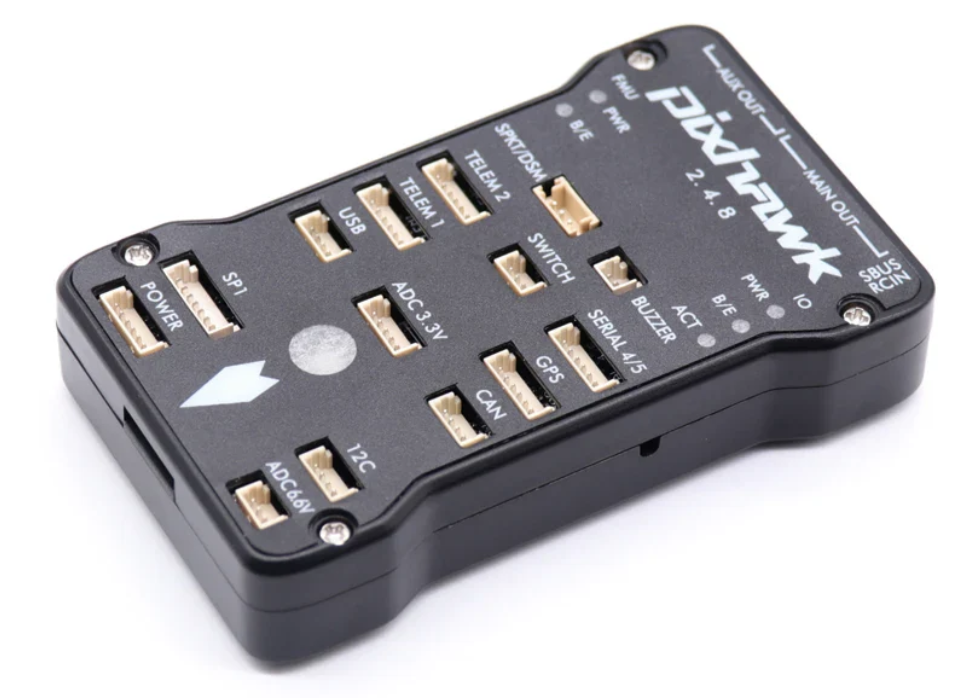
\includegraphics[width=0.4\textwidth]{Plataforma/pixhawk.png}
    \caption{Pixhawk embarcada na aeronave DH.}
    \label{fig:plataforma-avionica}
\end{figure}

\subsection{Sensores inerciais (acelerômetro e giroscópio)}

As grandezas inerciais provêm da unidade de medição inercial (IMU) integrada à controladora, um sensor InvenSense MPU-6000 que reúne, em um mesmo encapsulamento, um acelerômetro e um giroscópio de três eixos. O giroscópio fornece as velocidades angulares $p$, $q$ e $r$ no referencial do corpo, e o acelerômetro fornece as forças específicas $a_x$, $a_y$ e $a_z$, ambas registradas a aproximadamente $25$~Hz nos logs. Cabe distinguir essas taxas de registro da taxa de execução do laço de controle. Os $25$~Hz referem-se apenas à gravação dos dados, posteriormente reamostrados na grade comum de $10$~Hz empregada na identificação, conforme o Capítulo~\ref{chap:identificacao}. A essa taxa corresponde uma frequência de Nyquist de $5$~Hz: componentes espectrais acima desse limite tornam-se, após a amostragem, indistinguíveis de componentes de frequência mais baixa e distorcem o espectro do sinal amostrado, efeito conhecido como \textit{aliasing} \cite{Aguirre2015}. O projeto não incorre nesse problema por dois motivos. Primeiro, as dinâmicas de interesse concentram-se abaixo de $2$~Hz, atendendo ao critério de Nyquist com margem superior a duas vezes \cite{Jategaonkar2015}. Segundo, o conteúdo de alta frequência remanescente, como o ruído de vibração dos motores, é atenuado pela filtragem de Savitzky--Golay do tratamento de dados, e a análise espectral das manobras, apresentada no Capítulo~\ref{chap:identificacao}, confirma a energia concentrada em torno de $1$~Hz, sem componentes espúrias na banda de interesse.

Cabe reconhecer, contudo, o que a taxa dos dados limita: o alcance da própria identificação. Dados amostrados a $10$~Hz só revelam comportamento até a frequência de Nyquist de $5$~Hz e, na prática, as manobras de excitação concentram energia até cerca de $2$~Hz. O modelo identificado está, portanto, validado nessa faixa. Acima dela, ele não está incorreto, mas não verificado: dinâmicas mais rápidas, como eventuais modos de flexão estrutural, não são visíveis nos dados e, por consequência, não estão contidas no modelo. Essa limitação não compromete os resultados do trabalho por duas razões. As malhas de controle projetadas possuem banda passante em torno de $1$~Hz, dentro da faixa validada, e a dinâmica rápida relevante do laço, a do conjunto motor--ESC, foi caracterizada separadamente em bancada, com instrumentação dedicada (Apêndice~\ref{ap:bancada}).

O laço de controle não opera nessas taxas: o \textit{firmware} embarcado executa o controle de atitude a $400$~Hz, e as simulações deste trabalho atualizam o controlador a $100$~Hz, mais de cem vezes o polo dominante de malha fechada ($\omega_n = 6$~rad/s na atitude), razão que supera as recomendações práticas para a implementação digital de projetos em tempo contínuo.

O giroscópio apresenta ruído baixo: o \textit{datasheet} do MPU-6000 especifica densidade espectral de ruído de $0{,}005~^{\circ}/\mathrm{s}/\sqrt{\mathrm{Hz}}$ \cite{Invensense2013}, o que projeta, na banda de $12{,}5$~Hz dos registros, um ruído eficaz da ordem de $3\times10^{-4}$~rad/s. O valor observado em repouso nos logs, de aproximadamente $5\times10^{-4}$~rad/s, é coerente com essa especificação. O acelerômetro, por sua vez, carrega o ruído de vibração dos motores. É importante notar que a atitude $(\phi,\theta,\psi)$ não é medida diretamente: ela é estimada pelo EKF da controladora, combinando o giroscópio, o acelerômetro e o magnetômetro, com a guinada apoiada em um estimador dedicado. Essa característica está na origem da menor observabilidade do eixo de guinada, discutida nos capítulos seguintes.
